\documentclass[11pt]{article}
\usepackage{algorithm2e}
\usepackage[italian]{babel}
\usepackage[document]{ragged2e}
\usepackage{amsfonts, amssymb, amsmath}
\usepackage{cancel}
\usepackage{float}
\usepackage{mathtools}
\usepackage[margin=3cm]{geometry}

\tolerance=1
\emergencystretch=\maxdimen
\hyphenpenalty=10000
\hbadness=10000

\begin{document}
\begin{titlepage}
    \begin{center}
        \vspace*{1.5cm}
            
        \Huge
        \textbf{Tweet Analysis}
            
        \vspace{0.3cm}
        \LARGE
        Sprint 3\\[0.2em]
        \Large
        17 novembre 2022 -- 1 dicembre 2022

        \vspace{1.5cm}
          
        \begin{minipage}[t]{0.47\textwidth}
            \begin{center}
                \parbox{50mm}{\centering\large {\bf Cheikh Ibrahim $\cdot$ Zaid} \\[0.2em] PO Operativo \\[0.3em] Matricola: \texttt{0000974909}}\\[2em]
                \parbox{50mm}{\centering\large {\bf Lee $\cdot$ Qun Hao Henry} \\[0.2em] Developer \\[0.3em] Matricola: \texttt{0000990259}}
            \end{center}
		\end{minipage}
		\hfill
		\begin{minipage}[t]{0.47\textwidth}\raggedleft
            \begin{center}
                \parbox{50mm}{\centering\large {\bf Xia $\cdot$ Tian Cheng} \\[0.2em] Scrum master \\[0.3em] Matricola: \texttt{0000975129}}\\[2em]
                \parbox{50mm}{\centering\large {\bf Paris $\cdot$ Manuel} \\[0.2em] Developer \\[0.3em] Matricola: \texttt{0000997526}}
            \end{center}
		\end{minipage}  
            
        \vspace{6cm}
            
        Anno accademico\\
        $2022 - 2023$
            
        \vspace{0.8cm}
            
            
        \Large
        Corso di Ingegneria del Software\\
        Alma Mater Studiorum $\cdot$ Università di Bologna\\
            
    \end{center}
\end{titlepage}
\pagebreak


\section*{Sprint goal}
\justify
Per lo sprint è stata pianificata l'implementazione delle epiche riguardanti i giochi televisivi (L'Eredità e Reazione a Catena) e
l'inizio dell'epica riguardante lo scacchi.\\
In particolare sono state aggiunte le seguenti funzionalità:
\begin{itemize}
    \item Visualizzare gli utenti che tentano a indovinare la parola del giorno
    \item Visualizzare la parola vincente
    \item Visualizzare gli utenti che indovinano la parola
    \item Visualizzare la posizione degli utenti che tentano di indovinare
    \item Possibilità di muovere le proprie pedine su una scacchiera
\end{itemize}


\begin{figure}[H]
    \centering
    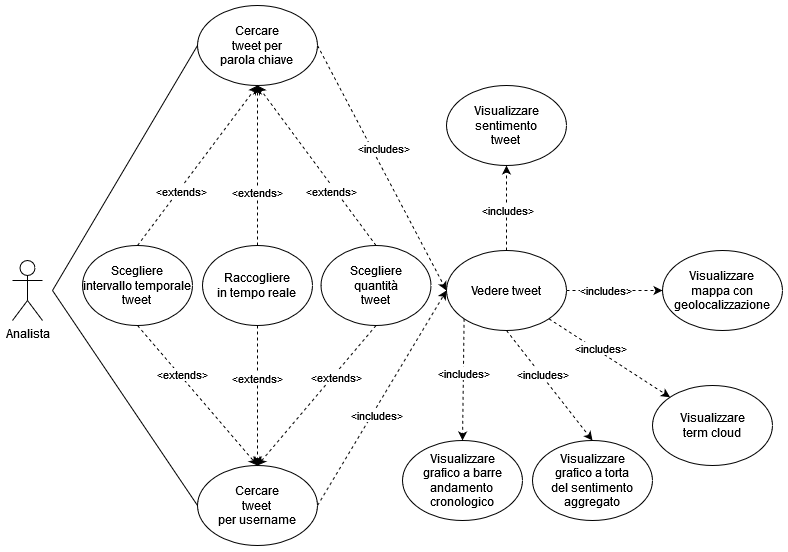
\includegraphics[width=12cm]{./img/tweet_usecase.png}
    \caption{Use case dell'analisi di Tweet (invariato rispetto allo sprint 2)}
\end{figure}

\begin{figure}[H]
    \centering
    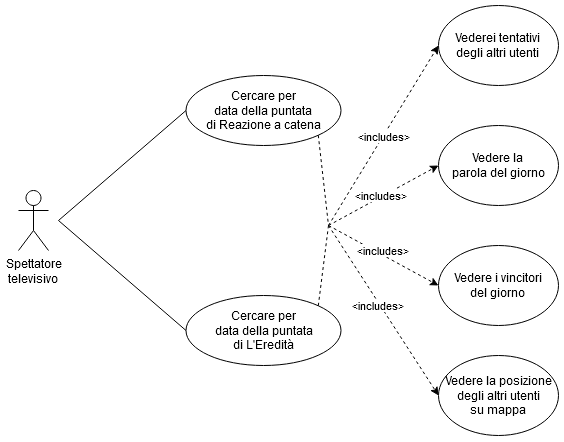
\includegraphics[width=10cm]{./img/tvgames_usecase.png}
    \caption{Use case dei giochi televisivi}
\end{figure}

\begin{figure}[H]
    \centering
    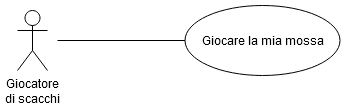
\includegraphics[width=6cm]{./img/chess_usecase.png}
    \caption{Use case degli scacchi}
\end{figure}

\newpage
\section*{Esito sprint}
Lo sprint è terminato con la conclusione di tutte le user stories pianificate.\\
Il lavoro è stato però distribuito in maniera disomogenea, infatti nella prima metà dello sprint non sono stati fatti progressi significativi,
mentre tutto il valore è stato portato nella seconda metà dello sprint.\\
Conseguentemente anche le ore di lavoro sono distribuite nel secondo periodo dello sprint.
\begin{figure}[H]
    \centering
    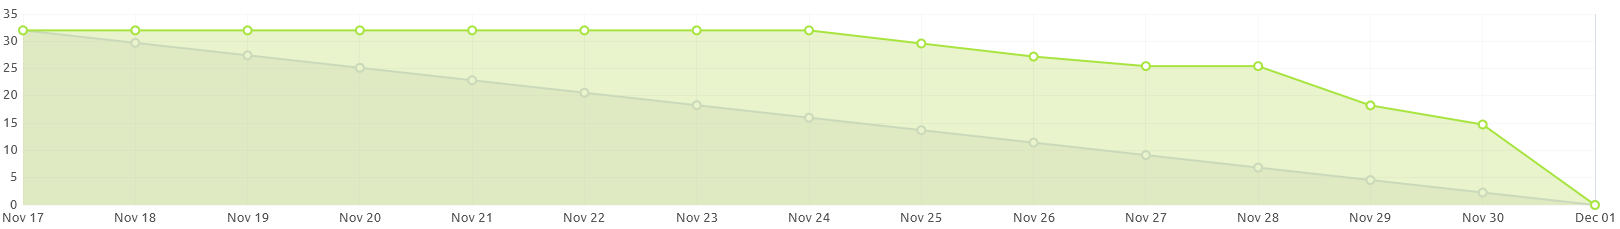
\includegraphics[width=\textwidth]{./img/burndown.png}
    \caption{Burndown generato da Taiga}
\end{figure}

\begin{figure}[H]
    \centering
    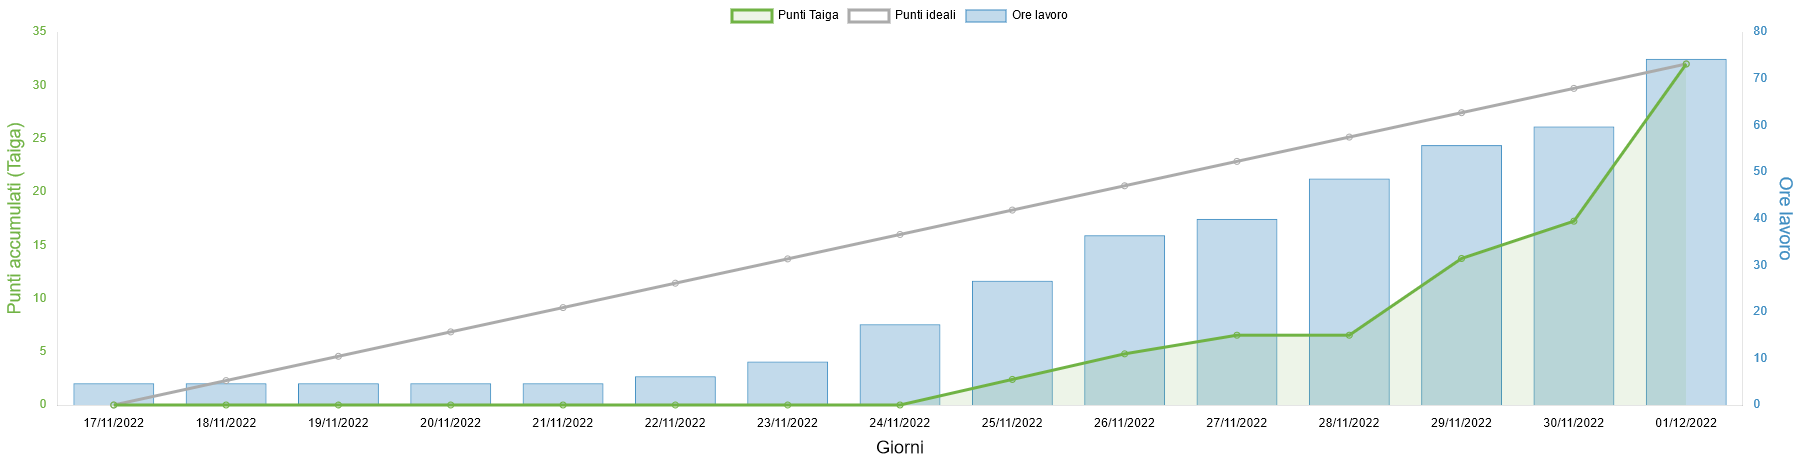
\includegraphics[width=\textwidth]{./img/worktime.png}
    \caption{Progresso dei punti (asse a sinistra) e ore di lavoro (asse a destra)}
\end{figure}

\section*{Sprint review}
Allo sprint review il cliente ha richiesto una revisione del grafico a barre sulla frequenza dei tweet, 
soprattutto in situazioni in cui sono presenti solo tweet di una giornata.

\newpage
\section*{Retrospettiva}
Dalla retrospettiva sono emerse le seguenti problematiche:
\begin{itemize}
    \item Abbiamo sottovalutato lo sprint e lavorato poco di conseguenza
    \item La DoD di alcune user stories risultavano ambigue
\end{itemize}
\begin{figure}[H]
    \centering
    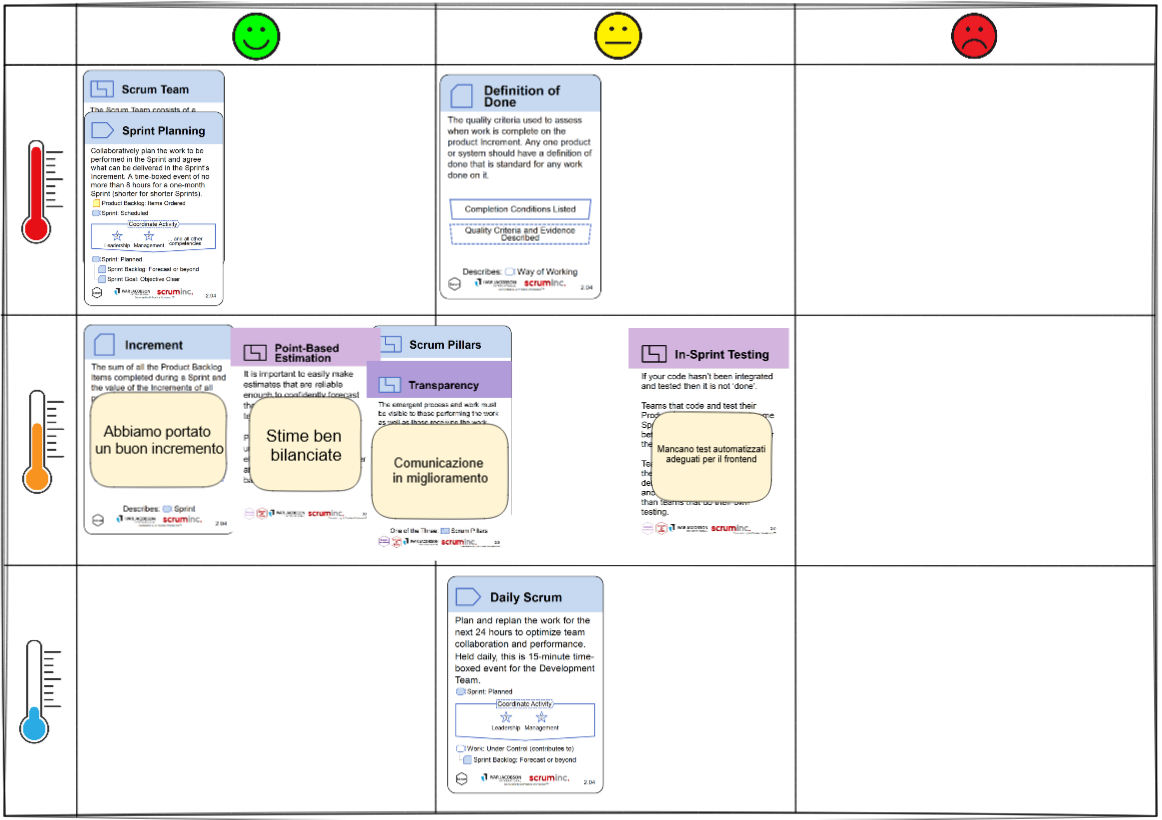
\includegraphics[width=12cm]{./img/retrospettiva.png}
    \caption{Carte Essence giocate alla retrospettiva}
\end{figure}


\end{document}

